\chapter{Gestión y planificación}

\section{Metodología de desarrollo}
Es bien sabido que en el ámbito del desarrollo software durante décadas se han dado problemas como el no cumplimiento ni de requisitos, ni de estimaciones de tiempo y recursos. Son el surgimiento de estos problemas a lo que evocó a la creación de metodologías de desarrollo con el objetivo de evitar o minimizar dichos problemas. Así que, una \textbf{metodología de desarrollo} se define como un de marco de trabajo utilizado con el fin de estructurar y controlar un proceso de desarrollo. \bigskip

A continuación se muestra una tabla con los dos grupos en los que puede ser una metodología de desarrollo clasificada junto con sus respectivas diferencias:

\begin{table}[H]
\begin{tabular}{|l|l|}
\hline
\rowcolor[HTML]{EFEFEF} 
\multicolumn{1}{|c|}{\cellcolor[HTML]{EFEFEF}Metodologías tradicionales}                                                                              & \multicolumn{1}{c|}{\cellcolor[HTML]{EFEFEF}Metodologías ágiles}                                               \\ \hline
\begin{tabular}[c]{@{}l@{}}La fase de test de la aplicación \\ es realizada sólo una vez tras \\ ser la fase de desarrollo \\ completada\end{tabular} & \begin{tabular}[c]{@{}l@{}}La fase de test de la aplicación\\ es un proceso realizado de \\ forma iterativa\end{tabular} \\ \hline
Sigue una organización lineal                                                                                                                         & Sigue una organización iterativa                                                                               \\ \hline
\begin{tabular}[c]{@{}l@{}}La participación del cliente\\ es menor\end{tabular}                                                                       & La participación del cliente es mayor                                                                          \\ \hline
\begin{tabular}[c]{@{}l@{}}Apoya un modelo de desarrollo\\ fijo\end{tabular}                                                                          & \begin{tabular}[c]{@{}l@{}}Apoya un modelo de desarrollo \\adaptable al cambio\end{tabular}                    \\ \hline
Difícil la adaptación al cambio                                                                                                                       & Fácil adaptación al cambio                                                                                     \\ \hline
Gestión de equipo grandes                                                                                                                             & Gestión de equipos pequeños                                                                                    \\ \hline
\end{tabular}
\label{tabla-metodologias}
\caption{Tabla de diferencias entre metodologías de desarrollo tradicional y ágil}
\end{table}

En lo que respecta a este proyecto, se reunen varios factores para inclinarnos por las metodologías ágiles:
\begin{itemize}
    \item El proyecto va dirigido a un cliente real, el cual puede añadir, modificar o eliminar cualquier requisito de los inicialmente planteados. Por tanto, hay que estar preparado para cualquier tipo de cambio.
    \item Se pretende hacer uso de tecnologías en las que no se tiene ninguna experiencia previa y esto puede conllevar a la ralentización de la planificación y en consecuencia a llevar a cabo modificaciones en ella.
    \item Como se indica en la Tabla \ref{tabla-metodologias} las metodologías ágiles son preferibles en equipos pequeños, estando en este caso el equipo formado por una sóla persona.
\end{itemize}

Una vez escogido el tipo de metodología, dentro de las metodologías ágiles nos encontramos con un amplio abanico de marcos de trabajo: SCRUM, eXtreme Programming, Kanban, Crystal Clear,etc. Se han tenido en consideración las dos primeras ya que de acuerdo al artículo \textit{''Organizational issues in embracing Agile methods: an empirical assessment''} de Alok Mishra et al. \cite{mishra2021organizational} las dos metodologías ágiles más populares actualmente son Scrum y eXtreme Programming y en consecuencia esto significa que han sido mayormente testeadas en distintas empresas y hay una mayor cantidad de documentación sobre ellas. Teniendo en cuenta la comparativa realizada por Juan Camilo Salazar et al. \cite{salazar2018scrum} de SCRUM y XP la poca disponibilidad del cliente, el tiempo de tan sólo 3 meses del que se dispone, la posible aparición de los riesgos expuestos en la Sección \ref{riesgos}  se concluye que XP resulta muy poco viable para este proyecto, no sólo por su poca flexibilidad, sino también porque requiere de trabajo en pareja y en este proyecto sólo participa una persona. Así pues, SCRUM es el marco de trabajo ideal para la naturaleza de este proyecto. \bigskip

En la siguiente Sección \ref{scrum} se explica de forma detallada qué es SCRUM y su adaptación al proyecto.

\subsection{SCRUM} \label{scrum}

\begin{figure}[H]
    \centering{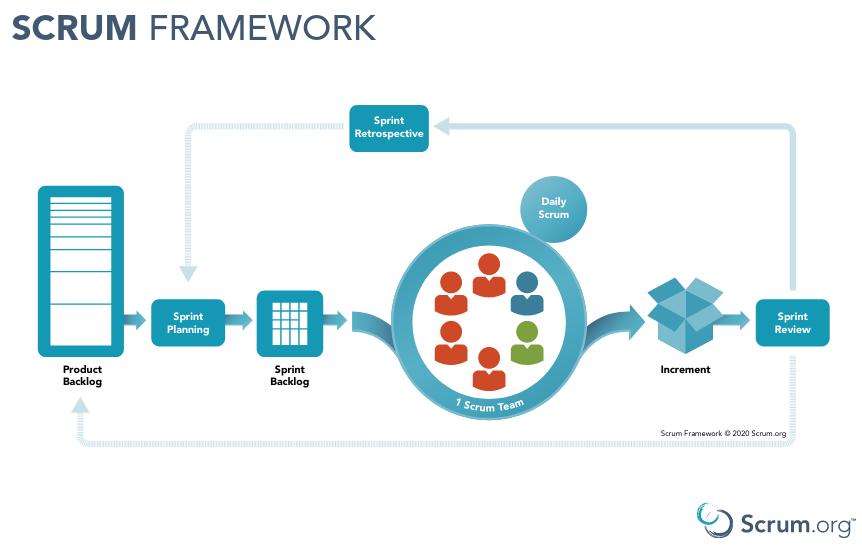
\includegraphics[scale=0.3]{doc/imagenes/scrum-esquema.png}}
    \caption{Esquema del marco de trabajo de SCRUM}
    \label{fig:scrum-esquema}
\end{figure}

La metodología de desarrollo ágil SCRUM (Figura \ref{fig:scrum-esquema}, imagen tomada de scrum.org \footnote{\url{https://www.scrum.org/}}), es de las metodologías de desarrollo más utilizadas en la actualidad, de hecho empresas de gran calibre como Movistar, Google, Vodafone, Electronic Arts... utilizan dicha metodología. \bigskip

Siguiendo el libro de Alonso Álvarez García et al. ''Métodos ágiles y Scrum'' \cite{Gomez2017-id}, ¿qué es SCRUM? Es un marco de trabajo para el desarrollo de proyecto caracterizado por ser iterativo e incremental, así como adaptativo pues no sigue un plan lineal, sino una adaptación continua. Sus principios son la \textbf{transparencia}, la \textbf{inspección} y la \textbf{adaptación} cumpliendo con los valores de mejora continua, compromiso, calidad, simplicidad, respeto, coraje, ritmo y responsabilidad. \bigskip

Sabiendo previamente que un \textbf{Sprint} es un intervalo de tiempo comprendido entre 1 a 4 semanas, durante el que se crea un incremento del producto del proyecto ''terminado'' y utilizable, SCRUM se compone de los siguientes elementos:

\begin{itemize}
    \item \textbf{Artefactos}:
    \begin{itemize}
        \item \textbf{Pila del producto (Product Backlog)}: Es una lista de requisitos que ha sido priorizada de todas las funcionalidades y características que ha de cumplir el producto. 
        \item \textbf{Pila del Sprint (Sprint Backlog)}: Es la selección de requisitos de la Pila del Producto, se compone de tareas de desarrollo que expresan los requisitos en lenguaje técnico.
    \end{itemize}
    \item \textbf{Reuniones}:
    \begin{itemize}
        \item \textbf{Planificación del Sprint}: Es una reunión previa antes del comienzo del Sprint en la que se determina el objetivo de éste y las tareas a desarrollar.
        \item \textbf{Reunión diaria}: Se trata de una reunión realizada diariamente en la que cada miembro del equipo expone las tareas realizadas, así como los obstáculos encontrados.
        \item \textbf{Revisión del Sprint}: Es una reunión que tiene lugar el último día del Sprint cuyo objetivo es el de obtener información sobre el estado del proyecto.
        \item \textbf{Retrospectiva del Sprint}: Al final de cada Sprint se realiza una reunión de retrospectiva en la que se identifican los puntos fuertes a mantener y débiles a mejorar del equipo durante el desarrollo.
    \end{itemize}
    \item \textbf{Roles}:
        \begin{itemize}
        \item \textbf{Propietario}: Es el representante del cliente, debe de conocer los requisitos del cliente y tener cierta experiencia con los métodos utilizados por el equipo. Se encarga de recolectar los requisitos del cliente, resolver dudas del Equipo de Desarrollo y de priorizar la Pila del Producto, así como de aceptar o rechazar el software realizado al final una iteración.
        \item \textbf{Director del proyecto}: Promueve los valores de Scrum, se asegura de que el equipo es totalmente funcional y es su escudo del resto del equipo ante amenazas externas. Se encarga de asegurar que el Propietario conozca cómo ordenar la Pila del Producto para maximizar el valor, de guiar y ayudar al Equipo de Desarrollo y motivar a que se realicen cambios que incrementen la productividad.
        \item \textbf{Equipo de desarrollo}: Se forma por un conjunto de profesionales que se ocupan de entregar un incremento del producto del proyecto ''terminado'' al final de cada Sprint. Normalmente un Equipo de Desarrollo se forma entre 5-9 personas.
    \end{itemize}
\end{itemize}

\subsection{Aplicación de SCRUM a este proyecto}
Debido a que el desarrollo del proyecto se hará de forma individual, se debe de hacer una adaptación de SCRUM a la metodología de trabajo que se va a llevar a lo largo del proyecto.

\begin{itemize}
    \item Como el Equipo de Desarrollo está compuesto por una sóla persona, las reuniones diaras son eliminadas.
    \item Al final de cada Sprint se acordará una reunión con la tutora en la que se hará una retrospectiva de éste. Además, durante todo el desarrollo se mantendrá el contacto para posibles dificultades o dudas.
\end{itemize}

\subsection{Especificación de requisitos}
En todo proyecto de desarrollo de un producto software es crucial una buena definición de los requisitos que deberá de cumplir éste para satisfacer totalmente las necesidades de sus usuarios. Debido a que como se ha explicado con anterioridad se está siguiendo la metodología de desarrollo ágil SCRUM, la definición de requisitos se hará a partir de historias de usuario. \bigskip

A continuación se muestran las historias de usuario identificadas para el desarrollo del proyecto. Cabe mencionar que, debido a su complejidad, las historias de usuario 2 (Tabla \ref{HU2}) y 3 (Tabla \ref{HU3}) han sido desglosadas en ''sub-historias de usuario''. 

\begin{table}[H]
\begin{tabular}{|
>{\columncolor[HTML]{CCCCCC}}l |l|}
\hline
\textbf{Identificación} & HU.1 - Sistema de inicio de sesión\\ \hline
\textbf{Descripción}    & Como usuario quiero poder iniciar y cerrar sesión de la plataforma. \\ \hline
\textbf{Aceptación}     & \begin{tabular}[c]{@{}l@{}}- El usuario intenta iniciar sesión, pero no está registrado \\ o las credenciales introducidas son erróneas y el sistema informa \\ de dicho error por la interfaz.\\ - Un usuario registrado introduce correctamente sus crendenciales y \\ es redirigido a la vista principal de la plataforma \\ obteniendo un JWT con fecha de expiración.\end{tabular}
\\ \hline
\textbf{Prioridad}     & \begin{tabular}[c]{@{}l@{}}Alta\end{tabular} \\ \hline
\textbf{Estimación}     & \begin{tabular}[c]{@{}l@{}}2 semanas\end{tabular} \\ 
\\ \hline\textbf{Tareas} & \begin{tabular}[c]{@{}l@{}}- Investigación sobre cómo implementar un sistema de login.\\ - Definir y crear el modelo de la base de datos de los usuarios.\\ - Definir un sistema jerárquico de roles.\\ - Implementar en Backend un sistema de login.\\ - Diseñar la interfaz del login.\\ - Implementar el diseño realizado en Frontend e implementar \\ las llamadas necesarias al Backend.\end{tabular} \\ \hline
\end{tabular}
\caption{HU.1 - Sistema de inicio de sesión}
\end{table}
\clearpage
\begin{table}[H]
\begin{tabular}{|
>{\columncolor[HTML]{CCCCCC}}l |l|}
\hline
\textbf{Identificación} & HU.2- Gestionar citas de un usuario \\ \hline
\textbf{Descripción}    & Como usuario quiero visualizar, crear, editar y borrar citas.  \\ \hline
\textbf{Aceptación}     & \begin{tabular}[c]{@{}l@{}}- Un usuario accede a la vista del ''Calendario'' y \\ visualiza las citas en las que éste dispone de permisos \\ para realizar cualquier operación CRUD.\end{tabular}         \\ \hline
\textbf{Prioridad}     & \begin{tabular}[c]{@{}l@{}}Alta\end{tabular} \\ \hline
\textbf{Estimación}     & \begin{tabular}[c]{@{}l@{}}2 semanas\end{tabular} \\ \hline 
\textbf{Tareas}         & \begin{tabular}[c]{@{}l@{}}- Investigación de Angular Schedule.\\ - Definir y crear el modelo de la base de datos de las citas.\\ - Diseñar la interfaz de la vista principal.\\ - Implementar los endpoints para operaciones CRUD sobre \\ citas en Backend utilizando el modelo de datos de Angular Schedule.\\ - Implementar el diseño realizado e implementar las llamadas a Backend.\end{tabular} \\ \hline
\end{tabular}
\caption{HU.2 - Gestionar citas de un usuario}
\label{HU2}
\end{table}

\begin{table}[H]
\begin{tabular}{|
>{\columncolor[HTML]{CCCCCC}}l |l|}
\hline
\textbf{Identificación} & HU.2.1- Visualización de las citas en el calendario  \\ \hline
\textbf{Descripción}    & \begin{tabular}[c]{@{}l@{}}Como usuario quiero visualizar en un calendario las \\ próximas citas y las pasadas.\end{tabular}  \\ \hline
\textbf{Prioridad}     & \begin{tabular}[c]{@{}l@{}}Alta\end{tabular} \\ \hline
\textbf{Estimación}     & \begin{tabular}[c]{@{}l@{}}1 semana\end{tabular} \\ \hline 
\textbf{Aceptación}     & \begin{tabular}[c]{@{}l@{}}- Un usuario paciente entra a la vista de ''Calendario'' y \\ visualiza todas sus citas en \\ un calendario.\\ - Un usuario psicólogo entra a la vista de ''Calendario'' y \\ visualiza todas las citas\\ de sus pacientes en un calendario.\\ - Un usuario administrador entra a la vista ''Calendario'' y \\ visualiza todas las citas de todos los usuarios en un calendario.\\ - Un usuario pulsa sobre una cita y el diálogo aparece \\ con todos los campos rellenos asociados a esa cita.\end{tabular} \\ \hline
\textbf{Tareas} & \begin{tabular}[c]{@{}l@{}}- Investigación de Angular Schedule\\ - Definir y crear el modelo de la base de datos de las citas\\ - Diseñar la interfaz de la vista del calendario\\ - Implementar el diseño realizado\end{tabular}  \\ \hline
\end{tabular}
\caption{HU.2.1 - Visualización de las citas en el calendario}
\end{table}

\begin{table}[H]
\begin{tabular}{|
>{\columncolor[HTML]{CCCCCC}}l |l|}
\hline
\textbf{Identificación} & HU.2.2- Crear y editar una cita \\ \hline
\textbf{Descripción}    & Como usuario quiero crear y modificar una cita en el calendario \\ \hline
\textbf{Prioridad}     & \begin{tabular}[c]{@{}l@{}}Alta\end{tabular} \\ \hline
\textbf{Estimación}     & \begin{tabular}[c]{@{}l@{}}1 semana\end{tabular} \\ \hline 
\textbf{Aceptación}     & \begin{tabular}[c]{@{}l@{}}- Un usuario pulsa sobre la franja de un día del calendario \\ y se abre un diálogo con un formulario con los campos: paciente, \\ psicólogo, hora de inicio de la cita, hora de fin de la cita y observaciones.\\ - Un usuario paciente intenta editar los campos de paciente con \\ su nombre y psicólogo con el nombre de su psicólogo, pero no puede \\ porque está deshabilitado.\\ - Un usuario psicólogo intenta editar el campo de psicólogo con su \\ nombre, pero no puede porque está deshabilitado.\\ - Un usuario administrador intenta modificar todos los campos y estos \\ son modificados con éxito.\\ - Un usuario intenta modificar el día y/u hora mostrados de la cita con un \\ especialista a una cita que no se encuentra libre, se muestra un \\ mensaje informado de ello.\\ - Se pulsa sobre el botón de guardado, el diálogo se cierra y una nueva cita \\ aparece en el calendario.\\ - Se pulsa sobre el botón de ''Cancelar'' y el diálogo se cierra.\end{tabular} \\ \hline
\textbf{Tareas}         & \begin{tabular}[c]{@{}l@{}}- Implementar los endpoints crear y editar citas en Backend \\ utilizando el modelo de datos de Angular Schedule.\\ - Implementar las llamadas a Backend en Frontend.\\ - Implementar el diálogo de creación/edición de citas en Frontend.\end{tabular}      \\ \hline
\end{tabular}
\caption{HU.2.2 - Crear y editar una cita }
\end{table}

\begin{table}[h]
\begin{tabular}{|
>{\columncolor[HTML]{CCCCCC}}l |l|}
\hline
\textbf{Identificación} & HU.2.3- Eliminar las citas de un usuario \\ \hline
\textbf{Descripción}    & Como usuario quiero eliminar una cita  \\ \hline
\textbf{Prioridad}     & \begin{tabular}[c]{@{}l@{}}Alta\end{tabular} \\ \hline
\textbf{Estimación}     & \begin{tabular}[c]{@{}l@{}}1 día\end{tabular} \\ \hline 
\textbf{Aceptación}     & \begin{tabular}[c]{@{}l@{}}- Se pulsa el botón de borrado de una cita existente, \\ se abre un diálogo preguntando si el usuario está seguro de la \\ acción, pulsa sí, el diálogo se cierra y ésta es eliminada del calendario.\\ - Se pulsa el botón de borrado de una cita existente, se abre un\\ diálogo preguntando si el usuario está seguro de la acción, pulsa no \\ y el diálogo se cierra sin tener efecto alguno.\end{tabular} \\ \hline
\textbf{Tareas}         & \begin{tabular}[c]{@{}l@{}}- Implementar el endpoint para eliminar citas en Backend.\\ - Implementar las llamadas a Backend en Frontend.\\ - Implementar el diálogo para confirmar el borrado de una cita en Frontend.\end{tabular} \\ \hline
\end{tabular}
\caption{HU.2.3 - Eliminar las citas de un usuario }
\end{table}

\begin{table}[H]
\begin{tabular}{|
>{\columncolor[HTML]{CCCCCC}}l |l|}
\hline
\textbf{Identificación} & HU.3- Gestión de los usuarios de la plataforma  \\ \hline
\textbf{Descripción}    & \begin{tabular}[c]{@{}l@{}}Como administrador quiero poder consultar, añadir, \\ modifcar y borrar usuarios de la plataforma.\end{tabular}                \\ 
\hline
\textbf{Prioridad}     & \begin{tabular}[c]{@{}l@{}}Alta\end{tabular} \\ \hline
\textbf{Estimación}     & \begin{tabular}[c]{@{}l@{}}2 semanas\end{tabular} \\ \hline 
\textbf{Aceptación}     & \begin{tabular}[c]{@{}l@{}}· Al pulsar sobre la sección de ''Pacientes'' del menú lateral, se navegará a una \\ nueva vista en la que se mostrará un listado de los pacientes de la clínica.\\ · Al pulsar sobre la sección de "Psicólogos" del menú lateral, \\ se navegará a una nueva vista en la que se mostrará un listado \\ de los psicólogos de la clínica.\\ ·Al pulsar sobre el botón de editar se mostrará un diálogo \\ con los campos del usuario a editar.\\ · Un campo del diálogo de editar un usuario se deja en \\ blanco y se informa del error.\\ · Todos los campos están rellenados y se pulsa sobre el botón \\ de guardado, el diálogo se cierra y la información del usuario \\ queda actualizada.\\ · Se pulsa sobre el botón de cancelar del diálogo y éste se cierra \\ sin haberse producido ningún efecto en la información del usuario.\\ · Se pulsa sobre el botón de eliminar, un diálogo es mostrado \\ preguntando si el usuario está seguro de dicha acción, se pulsa sí, el diálogo\\  se cierra y el usuario seleccionado es eliminado del listado, así como sus citas.\\ · Se pulsa sobre el botón de eliminar, un diálogo es mostrado\\  preguntando si el usuario está seguro de dicha acción, se pulsa ''Cancelar'' \\ y el diálogo se cierra sin tener ningún efecto.\end{tabular} \\ \hline
\textbf{Tareas}         & \begin{tabular}[c]{@{}l@{}}· Implementación de endpoints CRUD para los usuarios de la plataforma.\\ · Diseñar la vista del listado del personal\\ · Diseñar la vista del listado de pacientes.\\ · Implementar los diseños de las vistas anteriores.\end{tabular}            \\ \hline
\end{tabular}
\caption{HU.3- Gestión de los usuarios de la plataforma }
\label{HU3}
\end{table}

\begin{table}[H]
\begin{tabular}{|
>{\columncolor[HTML]{CCCCCC}}l |l|}
\hline
\textbf{Identificación} & HU.3.1- Crear y editar usuarios en la plataforma               \\ \hline
\textbf{Descripción}    & \begin{tabular}[c]{@{}l@{}}Como administrador quiero poder consultar, añadir, \\ modifcar y borrar usuarios de la \\ plataforma.\end{tabular}      \\ \hline
\textbf{Prioridad}     & \begin{tabular}[c]{@{}l@{}}Alta\end{tabular} \\ \hline
\textbf{Estimación}     & \begin{tabular}[c]{@{}l@{}}1 semana\end{tabular} \\ \hline 
\textbf{Aceptación}     & \begin{tabular}[c]{@{}l@{}}- Al pulsar sobre el botón de crear usuario se mostrará \\ un diálogo con todos los campos asociados a un usuario.\\ - Al pulsar sobre el botón de editar se mostrará un diálogo \\ con los campos del usuario a editar.\\ - Un campo del diálogo de editar un usuario se deja en blanco \\ y se informa del error.\\ - Todos los campos están rellenados y se pulsa sobre el botón de \\ guardado, el diálogo se cierra y la información del usuario \\ queda actualizada.\\ - Se pulsa sobre el botón de cancelar del diálogo y éste se cierra \\ sin haberse producido ningún efecto en la información del usuario.\end{tabular} \\ \hline
\textbf{Tareas}         & \begin{tabular}[c]{@{}l@{}}- Implementación de endpoints para crear y \\ editar usuarios en la plataforma.\\ - Implementar las llamadas en Front al Backend \\ para crear y editar usuarios.\end{tabular}    \\ \hline
\end{tabular}
\caption{HU.3.1 - Crear y editar usuarios en la plataforma  }
\end{table}

\begin{table}[H]
\begin{tabular}{|
>{\columncolor[HTML]{CCCCCC}}l |l|}
\hline
\textbf{Identificación} & HU.3.2- Borrar usuarios de la plataforma \\ \hline
\textbf{Descripción}    & \begin{tabular}[c]{@{}l@{}}Como administrador quiero poder borrar usuarios de la \\ plataforma.\end{tabular}  \\ \hline
\textbf{Prioridad}     & \begin{tabular}[c]{@{}l@{}}Alta\end{tabular} \\ \hline
\textbf{Estimación}     & \begin{tabular}[c]{@{}l@{}}1 semana\end{tabular} \\ \hline 
\textbf{Aceptación}     & \begin{tabular}[c]{@{}l@{}}- Se pulsa sobre el botón de eliminar, un diálogo es \\ mostrado preguntando si el usuario está seguro de \\ dicha acción, se pulsa sí, el diálogo se cierra y el \\ usuario seleccionado es eliminado del listado. \\ - Se pulsa sobre el botón de eliminar, un diálogo es \\ mostrado preguntando si el usuario está seguro de dicha \\ acción, se pulsa ''Cancelar'' y el diálogo se cierra sin \\ tener ningún efecto.\end{tabular} \\ \hline
\textbf{Tareas}         & \begin{tabular}[c]{@{}l@{}}- Implementación del endpoint encargado de borrar \\ usuarios de la plataforma.\\ - Implementar la llamada al endpoint para eliminar \\ usuarios en Frontend\end{tabular}    \\ \hline
\end{tabular}
\caption{HU.3.2 - Borrar usuarios de la plataforma }
\end{table}

\begin{table}[H]
\begin{tabular}{|
>{\columncolor[HTML]{CCCCCC}}l |l|}
\hline
\textbf{Identificación} & HU.4- Gestionar el perfil de un usuario \\ \hline
\textbf{Descripción}    & Como usuario quiero gestionar mi perfil de la plataforma \\ 
\hline
\textbf{Prioridad}     & \begin{tabular}[c]{@{}l@{}}Media\end{tabular} \\ \hline
\textbf{Estimación}     & \begin{tabular}[c]{@{}l@{}}2 semanas\end{tabular} \\ \hline 
\textbf{Aceptación}     & \begin{tabular}[c]{@{}l@{}}- Al pulsar sobre la opción de ''Perfil'' del menú lateral \\ se abre un diálogo en el que se muestran el email, nombre \\, rol del usuario es mostrado y un formulario para cambiar la contraseña actual.\\ - El usuario intenta pulsar sobre rol pero no puede editarlo.\\ - El usuario intenta pulsar sobre email o nombre y el campo es editable.\\. El usuario introduce la nueva contraseña, pulsa \\ sobre el botón de guardardado y la contraseña es actualizada.\\ - El usuario pulsa sobre cambiar contraseña y un diálogo es mostrado \\ con un formulario para introducir su contraseña actual y la nueva. \end{tabular} \\ \hline
\textbf{Tareas}         & \begin{tabular}[c]{@{}l@{}}- Diseñar la vista de
perfil\\ -  Añadir endpoint para cambiar
la contraseña de un usuario en
backend\\ - Implementar en Frontend el diseño realizado\end{tabular}  \\ \hline
\end{tabular}
\caption{HU.4 - Gestionar el perfil de un usuario  }
\end{table}


\subsection{Requisitos adicionales}
\begin{itemize}
    \item \textbf{Usabilidad}: La plataforma deberá de ser intuitiva, con flujos de usuario sencillos.
    \item \textbf{Seguridad}: La plataforma deberá de garantizar la privacidad de los datos proporcionados por los usuarios.
    \item \textbf{Compatibilidad}: El código podrá ser portable y funcionar correctamente en cualquier sistema operativo.
    \item \textbf{Costo}: Se procurará que el coste del proyecto sea el más bajo posible
    \item \textbf{Mantenimiento}: Para su posterior mantenimiento las partes de código más complejas deberán de haber sido comentadas.
\end{itemize}{}


\section{Gestión de la configuración}
En esta sección se indicará cómo se procederá para la gestión de la configuración de todos los elementos pertenecientes a este proyecto. Debido a que los elementos de trabajo que conforman el proyecto son el código y la documentación, a continuación se explicará la gestión de cada uno por separado.

\subsection{Gestión del código}
Para la gestión del código, control de versines del mismo y para evitar cualquier posible pérdida se hará uso de Github y de Git. Para ello, se procederá a crear un repositorio en local vinculado al repositorio en remoto de Github que previamente habrá sido creado con el nombre \textbf{TFG}\footnote{\url{https://github.com/ins426/TFG}}. En el \textit{README} \footnote{\url{https://github.com/ins426/TFG#bachelors-thesis-dayday-appointment-scheduling-for-clinics}} de dicho repositorio se encontrarán los enlaces a los dos repositorios que contendrán el código de la plataforma, uno para el backend llamado \textbf{TFG-backend} \footnote{\url{https://github.com/ins426/TFG-backend}} y otro para el frontend llamado \textbf{TFG-frontend}\footnote{\url{https://github.com/ins426/TFG-frontend}}. Al igual que con el repositorio global, también se tendrá un repositorio en local para cada uno. \bigskip

En cuanto a las herramientas utilizadas en cada repositorio, el backend será implementado en el lenguaje de programación JavaScript haciendo uso de Node.js y Express para construir la API. Por otro lado, el frontend será implementado en el lenguaje TypeScript haciendo uso de Angular y se utilizarán HTML, SCSS, Angular Material, Angular Flex-Layout y RxJS para construir la interfaz. \bigskip

Todas las herramientas mencionadas anteriormente son más adelante explicadas en la Sección \ref{recursos-software}.

\subsection{Gestión de la documentación}
En lo que respecta a la gestión de la documentación, ésta será redactada en la plataforma Overleaf en LaTeX y cada entrega realizada a la tutora será alojada en el repositorio \textit{TFG} de Github del proyecto. Debido a que Overleaf requiere de un plan de pago para llevar a cabo la sincronización con Github, se ha utilizado el repositorio en local creado para llevar a cabo dicha sincronización con el repositorio en remoto.

\section{Gestión del tiempo} \label{gestion-tiempo}
Para alcanzar con los objetivos propuestos del proyecto se han definido una serie de épicas y tareas asociadas a ellas:
\begin{itemize}
    \item \textbf{E.1} Estado del arte de la gestión de citas online:
    \begin{itemize}
        \item \textbf{T.1.1}: Entrevista con la clínica Carmen Verdejo para conocer su gestión actual de citas.
        \item \textbf{T.1.2}: Investigación sobre las herramientas utilizadas en la clínica Carmen Verdejo.
        \item \textbf{T.1.3}: Buscar y leer literatura sobre gestión de citas online.
        \item \textbf{T.1.4}: Investigación de soluciones genéricas dedicadas a planificación.
        \item \textbf{T.1.5}: Investigación de soluciones específicas para la gestión de citas en centros sanitarios.
    \end{itemize}
    
    \item \textbf{E.2}: Implementación de un login para personal y pacientes:
    \begin{itemize}
        \item \textbf{T.2.1}: Investigación sobre cómo implementar un sistema de login.
        \item \textbf{T.2.2}: Definir y crear el modelo de la base de datos de los usuarios.
        \item \textbf{T.2.3}: Definir un sistema jerárquico de roles.
        \item \textbf{T.2.4}: Implementar en Backend un sistema de login.
        \item \textbf{T.2.5}: Diseñar la interfaz del login.
        \item \textbf{T.2.6}: Implementar el diseño realizado en T.2.3 en Frontend e implementar las llamadas al Backend.
    \end{itemize}
    
    \item \textbf{E.3}: Implementación de la vista principal:
    \begin{itemize}
        \item \textbf{T.3.1}: Investigar Angular Schedule de Syncfusion.
        \item \textbf{T.3.2}: Definir y crear el modelo de la base de datos de las citas.
        \item \textbf{T.3.3}: Diseñar la interfaz de la vista del calendario.
        \item \textbf{T.3.4}: Implementar el diseño realizado.
        \item \textbf{T.3.5}:  Implementar los endpoints crear y editar citas en Backend utilizando el modelo de datos de Angular Schedule de Syncfusion.
        \item \textbf{T.3.6}: Implementar las llamadas de creación y edición de citas a Backend en Frontend.
        \item \textbf{T.3.7}:  Implementar el diálogo de creación/edición de citas en Frontend.
        \item \textbf{T.3.8}: Implementar el endpoint para eliminar citas en Backend.
        \item \textbf{T.3.9}: Implementar el diálogo para confirmar el borrado de una cita en Frontend.
    \end{itemize}
    \item \textbf{E.4}: Implementación de las vistas del listado de personal y pacientes:
    \begin{itemize}
        \item \textbf{T.4.1}:  Implementación de endpoints para creación y edición de usuarios de la plataforma.
        \item \textbf{T.4.2}: Diseñar la vista del listado del personal y pacientes.
        \item \textbf{T.4.3}: Implementar las llamadas en frontend al backend para crear y editar usuarios.
        \item \textbf{T.4.4}: Implementar las vistas de los diseños de T.4.2.
        \item \textbf{T.4.5}: Implementar el endpoint encargado de borrar usuarios de la plataforma.
        \item \textbf{T.4.6}: Implementar la llamada al endpoint para eliminar usuario en Frontend.
    \end{itemize}
    \item \textbf{E.5}: Implementación de la vista de perfil:
    \begin{itemize}
        \item \textbf{T.5.1}: Diseñar la vista de perfil.
        \item \textbf{T.5.2}: Añadir endpoint de cambiar contraseña en el Backend.
        \item \textbf{T.5.3}: Implementar en Frontend el diseño de T.5.1. y conectarlo con el Backend
    \end{itemize}

    \item \textbf{E.6}: Implementación de pruebas:
    \begin{itemize}
        \item \textbf{T.6.1}: Hacer estudio de tecnologías para realizar las pruebas.
        \item \textbf{T.6.2}: Definición e implementación de las pruebas.
    \end{itemize}   

\end{itemize}

\subsection{Planificación temporal}
En el siguiente Diagrama de Gantt (Figura \ref{fig:gantt}) se recoge la temporización estimada del proyecto:

\begin{figure}[H]
    \centering{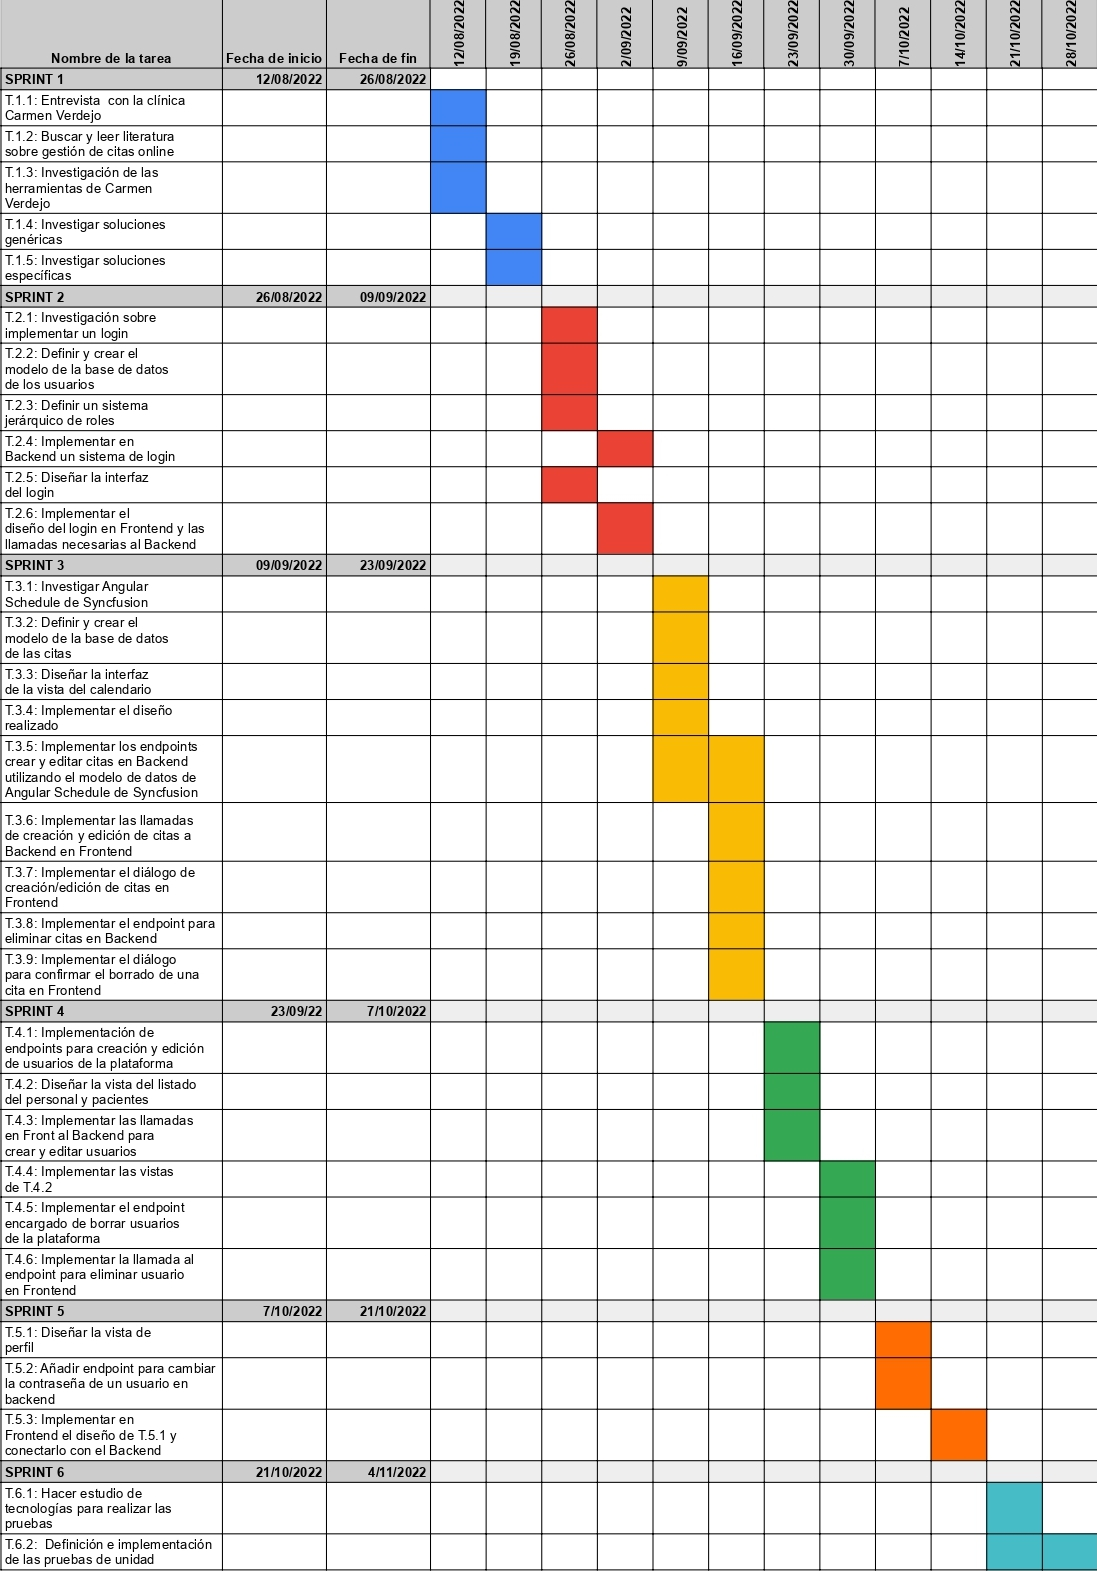
\includegraphics[scale=0.47]{doc/imagenes/gantt.jpg
    }}
    \caption{Diagrama de Gantt de la planificación temporal}
    \label{fig:gantt}
\end{figure}

Además de estas tareas, durante el desarrollo del proyecto se redactará toda la documentación correspondiente a éste.

\section{Gestión de recursos} \label{recursos}
\subsection{Recursos humanos}
\begin{itemize}
    \item \textbf{Dña. Rocío Celeste Romero Zaliz}, profesora del Departamento de Ciencias de la Computación e Inteligencia Artificial de la Universidad de Granada como tutora del proyecto.
    \item \textbf{Inés Nieto Sánchez}, estudiante del grado en Ingeniería Informática en la Escuela Técnica Superior de Ingenierías Informática y Telecomunicación.
\end{itemize}

\subsection{Recursos materiales} \label{materiales}
Los recursos utilizados para este Trabajo de Fin de Grado han sido muy pocos, en concreto sólo se ha utilizado el portátil personal:
\begin{itemize}
    \item \textbf{MSI Modern 14 A10M}: Se trata de un portatil de la marca MSI con un procesador Comet Lake i7-10510U con una memoria RAM de 16GB y una arquitectura de 64 bits. Todo el desarrollo del proyecto, así como la documentación correspondientes serán realizados haciendo uso de este portátil.
\end{itemize}
\subsection{Recursos software} \label{recursos-software}
En cuanto a los recursos software se ha optado por la utilización de software de código abierto y recurrido a las licencias gratuitas ofrecidas al estudiantado para disminuir lo máximo posible el coste del proyecto. A continuación se expone el listado de los recursos software utilizados:

\begin{itemize}
    \item \textbf{Elementary OS}: Se trata de una distribución de código abierto del sistema operativo Linux.
    \item \textbf{WebStorm}: Es una IDE dedicada sobretodo al desarrollo web en JavaScript y Typesrcipt. Pertenece a la empresa de desarrollo software JetBrains y a pesar de que todas las IDEs desarrolladas por JetBrains son de pago, se hará uso de la licencia gratuita ofrecida a estudiantes.
    \item \textbf{Git}: Se trata de un software de código abierto para el control de versiones de un proyecto.
    \item \textbf{Github}: Es una plataforma cuyo servicio es el de alojar el sistema de control de versión Git.
    \item \textbf{Docker}: Es una herramienta de código abierto diseñada con objeto de automatizar el despliegue de aplicaciones en contenedores software.
    \item \textbf{Docker Compose}: Es una herramienta dedicada a la orquestación de contenedores Docker.
    \item \textbf{Node.js}: Es un entorno de código abierto utilizado para hacer uso de JavaScript ejecutar JavaScript fuera del navegador.
    \item \textbf{Express.js}: Se trata de un framework de código abierto de backend para aplicaciones web de Node.js para construir APIs RESTful.
    \item \textbf{Angular}: Es un framework de código abierto desarrollado por Google utilizado para crear aplicaciones web y móviles.
    \item \textbf{MongoDB Atlas}: Es un servicio sobre gestión de base de datos MongoDB basado en la nube. Se hará uso de su prueba gratis en la que se permite la creación de una base de datos gratuita. 
    \item \textbf{Postman}: Se trata de una plataforma API para construir y crear APIs. Será utilizada para probar la funcionalidad de los endpoints de la aplicación.
    \item \textbf{AWS}: Es un conjunto de servicios de computación en la nube. Se hará uso del servicio EC2 y Route 53 para hacer el despliegue. Estos servicios tienen un coste en un función de sus horas de uso. El tipo de instancia escogida que se explicará en el Capítulo \ref{despliegue} tiene un precio de 0,047€/hora. Se prevee un uso máximo de la instancia de unas 10 horas por lo que aproximadamente su coste máximo será de 0.47€.
    \item \textbf{Cloudfare}: Como la anterior herramienta, formará parte del despliegue y será utilizada para comprar un dominio para la plataforma. En este caso el dominio escogido tuvo un precio de 4€.
    \item \textbf{Let's Encrypt}: Es una autoridad de certificación que ofrece de manera gratis certificados SSL.
\end{itemize}

\subsection{Recursos  de comunicación y documentación}
Para la correcta evolución del proyecto se han de hacer uso de recursos para la comunicación entre sus participantes, así como el uso de herramientas utilizadas para la documentación del mismo.

\begin{itemize}
    \item \textbf{Overleaf}: Es un editor gratuito de LaTeX en la nube, utilizado para la documentación del proyecto.
    \item \textbf{Jira}: Software dedicado a la gestión de proyectos, se utilizará su plan grautito para la gestión del proyecto siguiendo una metodología SCRUM.
    \item \textbf{Visual Paradigm}: Es una aplicación software cuyo objetivo es el de modelado de sistemas de información y procesos de gestión de desarrollo. Se trata de una herramienta de pago, pero la Universidad de Granada ofrece a su estudiantado licencias gratuitas.
    \item \textbf{Draw.io}: Es un software online gratuito desarrollado por Google utilizado para la creación de diagramas y esquemas.
    \item \textbf{Figma}: Herramienta de diseño para crear aplicaciones, webs, logos...Su paquete gratis será utilizado para la creación de los wireframes y mockups de la plataforma.
    \item \textbf{Milanote}: Es un software gratis en la nube diseñado para organizar ideas y proyectos en tableros visuales.
    \item \textbf{Google slides}: Es una herramienta desarrollada por Google para la creación y edición de presentaciones. Será utilizada para la elaboración de la presentación del proyecto.
    \item \textbf{Google meet}: Es un servicio de videoconferencia desarrollado por Google.
    \item \textbf{Correo UGR}: Es un servicio de correo electrónico de la UGR.
    \item \textbf{Clockify}: Es una herramienta para dejar registro de las horas trabajadas en un proyecto.
\end{itemize}

\section{Gestión de costes}
En esta sección se elaborará un presupuesto de acuerdo a los recursos explicados en la Sección \ref{recursos} junto con los costes adicionales que supone el desarrollo del proyecto.

\subsection{Costes de recursos humanos}
Para los costes de recursos humanos, hemos de tener en cuenta que el equipo de desarrollo está formado por una persona que tomará el rol de Ingeniera Informática. Para estimar el coste del trabajo de dicho rol a continuación se hará un desglose del número de horas totales a trabajar y su coste. \bigskip

El proyecto se encuentra planteado para ser realizado en un período de 3 meses, es decir, 12 semanas. 

\begin{center}
$Dias\ naturales\ =\ 3\ meses\ *\ 30\ dias / mes\ =\ 90\ dias$
\end{center}

A este número de días naturales habrá que descontarle fines de semana:

\begin{center}
$Dias\ no \ laborales\ =\ 3\ meses\ *\ 8\ dias / mes\ =\ 24\ dias$
\end{center}

Resultando ser los días laborales invertidos en el desarrollo del proyecto los siguientes:

\begin{center}
$Dias\ laborales\ =\ 90\ dias\ -\ 24\ dias =\ 66 \ dias$
\end{center}

En cuanto a las horas trabajadas, una jornada laboral completa se constituye de 40 horas semanales. Sin embargo, debido a que la estudiante trabaja en paralelo con una jornada parcial durante la realización del proyecto, las horas semanales dedicadas son reducidas a 30 horas distribuidas en 6 horas diarias. Por tanto, el total de horas trabajadas es el siguiente:

\begin{center}
$Horas\ laborales\ =\ 66\ dias\ *\ 6 \ horas\ día = \ 396 \ horas$
\end{center}

Después de haber obtenido las horas laborales totales, el salario como ingeniero informático se ha obtenido en base al salario anual indicado por la Universidad Alfonso X El Sabio \footnote{\url{https://www.uax.com/blog/ingenieria/cuanto-cobra-un-ingeniero-informatico}}. Según la universidad madrileña el salario de un ingeniero informático con menos de 3 años de experiencia gana aproximadamente 20.450 euros anuales, en otras palabras, 1.704 euros mensuales brutos que son 9,68 euros/hora. Así pues los costes de recursos humanos totales son:

\begin{center}
$Costes\ de \ recursos \ humanos \ =\ 396\ horas\ *\ 9.68 \ euros\ hora = \ 3.833,28 \ euros$
\end{center}

Sin embargo, se utilizó la herramienta Clockify para hacer un registro de las horas invertidas en el proyecto (Figura \ref{fig:clockify}), que como se ve finalmente fueron 413 horas. Por ello los costes de recursos humanos reales han sido:

\begin{center}
$Costes\ de \ recursos \ humanos \ reales \ =\ 413\ horas\ *\ 9.68 \ euros\ hora = \ 3997,84 \ euros$
\end{center}

\begin{figure}[H]
    \centering{
\includegraphics[scale=0.4]{doc/imagenes/clockfy.png}}
    \caption{Registro de horas trabajas en el proyecto en Clockify}
    \label{fig:clockify}
\end{figure}

\subsection{Costes de recursos materiales}
Una vez hemos calculado los costes de recursos humanos, es momento de calcular los costes de recursos materiales. Para su cálculo se deberá de tener en cuenta que los recursos sufren de un fenómeno llamado \textit{depreciación} el cual hace que estos sean devaluados con el paso del tiempo. \bigskip

Como se ha expuesto en la sección \ref{materiales} sólo se utilizará una sóla herramienta, el portátil personal de la estudiente. Para calcular su actual precio se aplicará el método de depreciación lineal usado para conocer la reducción del valor de un bien. 

\begin{table}[]
\begin{tabular}{|l|l|l|l|l|}
\hline
\rowcolor[HTML]{CCCCCC} 
\cellcolor[HTML]{CCCCCC}\textbf{Recurso} & \textbf{\begin{tabular}[c]{@{}l@{}}Valor\\ inicial(€)\end{tabular}} & \textbf{\begin{tabular}[c]{@{}l@{}}Valor\\ residual(€)\end{tabular}} & \textbf{\begin{tabular}[c]{@{}l@{}}Antigüedad\\ (años)\end{tabular}} & \textbf{\begin{tabular}[c]{@{}l@{}}Valor\\ actual\\ (€)\end{tabular}} \\ \hline
\rowcolor[HTML]{FFFFFF} 
\textbf{Portátil personal}& 899 & 179,8 & 4 & 323,64  \\ \hline
\rowcolor[HTML]{FFFFFF} 
\textbf{TOTAL} & & & & 323,64  \\ \hline
\end{tabular}
\caption{Tabla de los costes materiales}
\end{table}

Para calcular la depreciación se deberá antes calcular el valor residual del dispositivo el cual es el valor que poseerá al final de la vida útil del mismo. Suponemos para ello, que la vida útil de un portátil es de 5 años: 

\begin{equation}
    Valor\ residual = \frac{Coste\ inicial}{Vida\ util\ (a\tilde{n}os)} = \frac{899 \ \EUR}{5 \ a\tilde{n}os} = 179,8\ \EUR{}
\end{equation}

 Una vez conocido el valor residual, la depreciación se calcula de la siguiente forma:
\begin{equation}
    Depreciacion = \frac{Coste \ inicial - Valor\ residual}{Vida\ util\ ( a\tilde{n}os)} = \frac{899\EUR \ - \ 179,8\EUR }{5 \ a\tilde{n}os} = 143,84\ \EUR{}
\end{equation}

\subsection{Costes de recursos software, comunicación y documentación}
Los costes referentes a los recursos software son de 4.47€, debido a los costes ya explicados de la instancia de 0.47€ de AWS y 4€ por el dominio de Cloudfare. El resto del coste de los recursos software es nulo puesto que todos son de código abierto, a excepción de WebStorm que no es gratutito, puesto que se hace uso de la licencia gratuita para estudiantes de JetBrains. Por otro lado, en lo que respecta a los recursos utilizados para la documentación y comunicación son totalmente gratuitos salvo Visual Paradigm el cual es utilizado por una licencia gratuita ofrecida por la UGR.


\subsection{Costes adicionales}
Dentro de los costes adicionales se encuentran aquellos costes que no se han nombrado en los apartados anteriores, pero han sido necesarios para el desarrollo del proyecto. Estos costes son correspondientes a la factura de la luz e Internet:


\begin{table}[H]
\centering
\begin{tabular}{cc}
\hline
\multicolumn{1}{l}{\textbf{Recurso}} & \multicolumn{1}{l}{\textbf{Importe (€/mes)}} \\ \hline
Luz                                  & 25                                           \\
Internet                             & 70                                           \\ \hline
\end{tabular}
\caption{Tabla de los costes adicionales}
\end{table}

\subsection{Presupuesto total}
En la siguiente tabla se presenta la visión global de los costes de este proyecto:

\begin{table}[H]
\centering
\begin{tabular}{lc}
\hline
\textbf{Recurso}                                                                                      & \multicolumn{1}{l}{  \textbf{Importe}} \\ \hline
\textbf{Costes de recursos humanos}                                                                   & \multicolumn{1}{l}{}                 \\
Trabajo autónomo                                                                                      & 3997,84€                            \\ \hline
\textbf{Costes de recursos materiales}                                                                & \multicolumn{1}{l}{}                 \\
Portátil personal                                                                                     & 323,64€                              \\ \hline
\textbf{Costes de recursos software}                                                                  & \multicolumn{1}{l}{}                 \\
Elementary OS                                                                                         & 0,0€                                 \\
WebStorm                                                                                              & 0,0€                                 \\
Git                                                                                                   & 0,0€                                 \\
Github                                                                                                & 0,0€                                 \\
Docker                                                                                                & 0,0€                                 \\
Docker Compose                                                                                        & 0,0€                                 \\
Node.js                                                                                                & 0,0€                                 \\
Angular                                                                                               & 0,0€

\\
MongoDBAtlas                                                                                               & 0,0€

\\
Postman                                                                                               & 0,0€  

\\
AWS                                                                                               & 0,47€ 

\\
Cloudfare                                                                                               & 4,0€  

\\
Let's Encrypt                                                                                               & 0,0€  

\\ \hline
\textbf{\begin{tabular}[c]{@{}l@{}}Costes de recursos de\\ comunicación y documentación\end{tabular}} & \multicolumn{1}{l}{}                 \\
Draw.io                                                                                               & 0,0€   
             \\
Figma                                                                                                & 0,0€  
\\
Milanote                                                                                              & 0,0€                                 \\
Overleaf                                                                                              & 0,0€                                 \\
Visual Paradigm                                                                                       & 0,0€                                 \\
Google Meet                                                                                           & 0,0€                                 \\
Correo UGR                                                                                            & 0,0€                                 \\
Clockify                                                                                                & 0,0€                                 \\ \hline
\textbf{Costes adicionales}                                                                           & \multicolumn{1}{l}{}                 \\
Factura de la luz                                                                                     & 25€ x 3 meses = 75€                                 \\
Factura de Internet                                                                                   & 70€  x 3 meses = 225€                                \\ \hline
\textbf{TOTAL}                                                                                        & \multicolumn{1}{l}{4.625,95€}       
\end{tabular}
\caption{Tabla del presupuesto total del proyecto}
\end{table}

\section{Gestión de riesgos} \label{riesgos}
Durante el desarrollo de todo proyecto se tiene siempre la posibilidad de que puedan manifestarse ciertas situaciones que supongan un obstáculo o incluso amenaza para su correcta evolución. Es por ello que por mínima que sea la posibilidad de que ocurran hay que estar preparado y para ello se debe de precisar un plan de actuación.

En esta sección se identificarán los posibles riesgos a correr durante el proyecto, sus causas y el plan de actuación en caso de ser materializados para solventar o reducir lo máximo posible su impacto. Posteriormente se hará una estimación de la probabilidad de aparición y del impacto que supone cada uno de ellos.

\subsection{Identificación de riesgos}
Los posibles riesgos para el desarrollo del proyecto identificados son mostrados en la siguiente tabla (Figura \ref{fig:riesgos}):

\begin{figure}[H]
    \centering{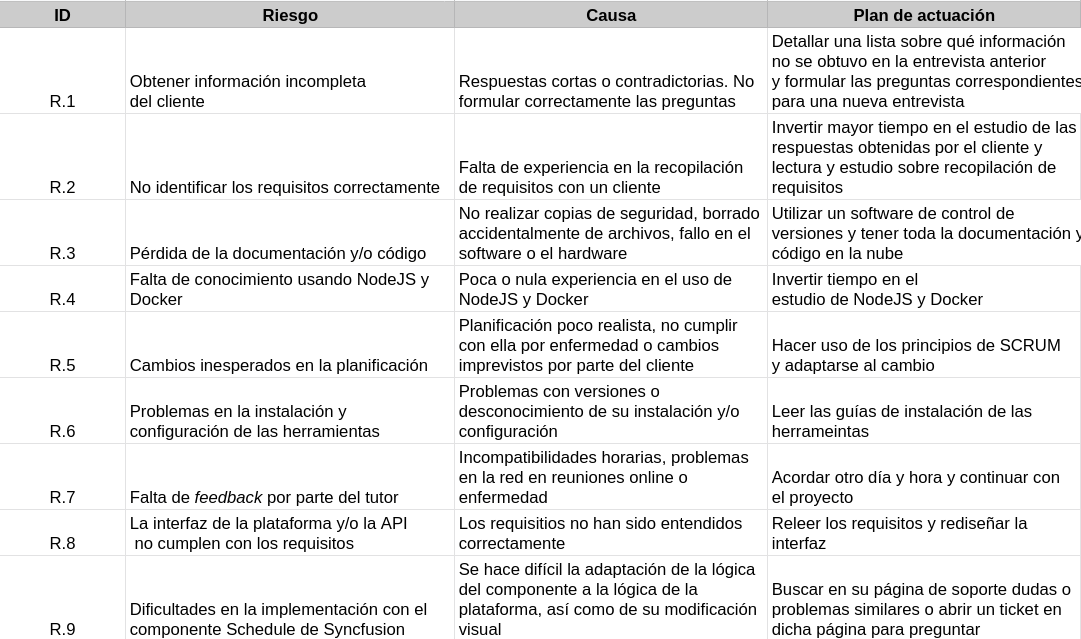
\includegraphics[scale=0.35]{doc/imagenes/riesgos.png}}
    \caption{Tabla de riesgos del proyecto}
    \label{fig:riesgos}
\end{figure}
\subsection{Análisis de riesgos}
Para analizar los riesgos expuestos anteriormente, se ha hecho uso de una matriz de probabilidad-impacto:

\begin{figure}[H]
    \centering{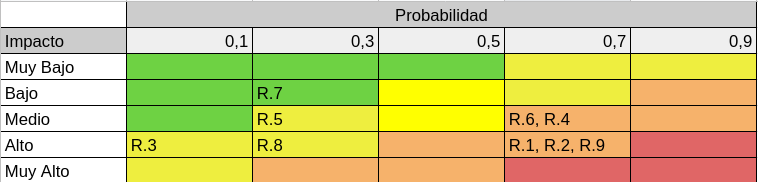
\includegraphics[scale=0.4]{doc/imagenes/analisis-riesgos.png}}
    \caption{Matriz de probabilidad-impacto de riesgos}
    \label{fig:analisis-riesgos}
\end{figure}

\subsection{Riesgos materializados} \label{riesgos-materializados}
Los riesgos surgidos durante el transcurro del desarrollo del proyecto han sido precisamanete los marcados con mayor probabilidad en la matriz de probabilidad-impacto \ref{fig:analisis-riesgos} (R.1, R.2, R.4 y R.6) . La falta de experiencia ante el reto que supone recoger información de un cliente ha provocado que surgieran numerosas dudas acerca de los requisitos del proyecto. A su vez la utilización de Docker y Node.js por primera vez ha evocado a invertir gran parte del tiempo del primer sprint en su instalación y estudio. Por último, el riesgo R.9 ha sido materializado, el cual ha resultado ser bastante crítico durante la realización del proyecto. Esto se debe a que supuso la alteración de la planificación debido a la caótica y escasa documentación presentada por Syncfusion para el componente del calendario y las largas esperas en su plataforma de soporte ante dudas planteadas. \bigskip

A pesar de la manifestación de los riesgos nombrados se ha sabido aplicar correctamente el plan de actuación previamente establecido para cada uno.